\documentclass[12pt,letter]{article}
\usepackage[moduleName=Jairasullator]{KautenjaDSP}
% import a debugging package to show the margin boxes
% \usepackage{showframe}
% set the graphics path to the img directory
\graphicspath{{img/}}

% algorithm2e stuff
% \SetKwInOut{Objects}{$\CKmatrix{O}$}
% \SetKwInOut{Weights}{$\CKvector{w}$}

\begin{document}
\titlePage{Jairasullator-Logo}{Jairasullator-Module}{KautenjaDSP}

% -------------------
% MARK: Overview
% -------------------

\section{Overview}

AY-3-8910 is an emulation of the General Instrument AY-3-8910 sound chip from
many Arcade games. The AY features three tone generators, each with an optional
noise effect.

AY-3-8910 provides the key features of the General Instrument AY-3-8910 chip,
namely,
\begin{itemize}
  \item \textbf{Triple pulse wave generator:} Triple 12-bit pulse waves with duty cycle of $50\%$
  \item \textbf{Noise generator:} Generate noise on each oscillator using the frequency knob for oscillator 3
  \item \textbf{Amplitude modulation:} Manual and CV control over the individual voice levels
  \item \textbf{Tone/Noise control:} CV and switch to control tone and noise for each oscillator
\end{itemize}

% -------------------
% MARK: Panel Layout
% -------------------

\clearpage
\section{Panel Layout}

\begin{figure}[!htp]
\centering
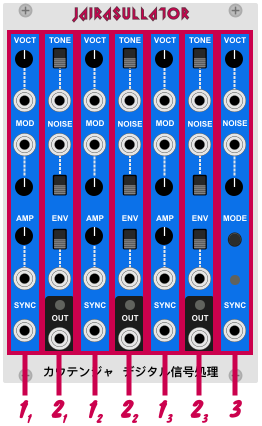
\includegraphics{Jairasullator-Manual}
\end{figure}

\begin{enumerate}
  \item Coarse frequency control over the four oscillators. The frequency of oscillator 3 also controls the period of the noise generator.
  \item $V$/Octave inputs for tone1, tone2, and tone3 waveform generators.
  \item linear CV frequency modulation for tone1, tone2, and tone3 waveform generators.
  \item On/off control over pulse generator (top) and noise generator (bottom) for each oscillator. The CV gate input goes high at $2V$. The toggle switch both acts as a basic switch and inverts the effect of the CV gate input.
  \item Coarse amplitude control over the oscillators using the 4-bit amplifier.When no input is connected, the slider controls the level from $0\%$ to $100\%$. When an input is connected, the slider acts as an attenuator.
  \item Channel outputs, ${\approx}10V_{pp}$.
\end{enumerate}

% -------------------
% MARK: References
% -------------------

\clearpage
\renewcommand\refname{References \& Acknowledgments}
\nocite{*}
\bibliographystyle{apalike}
\bibliography{references}

\end{document}
